% Modultest fugt og temp print

%tekst

I følgende afsnit testes fugt- og temperatursensoren sammen med lavpasfilter på det færdigudarbejdet PCB. Der testes for om temperatur og fugtighedsændringer registreres korrekt og om omregningen fra DC-niveau til værdi stemmer overens med scenariet i test. Scopbillederne er taget med et agilent oscilloskop.

SHT21p-sensoren udsender et PWM-signal med en frekvens på 120 hz i området 0V til VCC. Ud fra PWMen kan temperatur og fugtighed udregnes med følgende formler som er hentet fra databladet:

\begin{equation}
-6+125*duty cycle= fugtighed i \%
\end{equation}

\begin{equation}
-46.85+175.72*duty cycle= temperatur i grader celsius
\end{equation}

PWM-signalet bliver, gennem et 2. ordens lavpasfilter, midlet til en DC. Ud fra denne DC-
og VCC-værdi beregnes fugtigheden og temperaturen ved følgende formler.


\begin{equation}
-6+125*\frac{målt DC}{Vcc}= fugtighed i \%
\end{equation}

\begin{equation}
-46.85+175.72*\frac{målt DC}{Vcc}=temperatur i grader celsius
\end{equation}

Sensoren er forsynet med 3,3V men grundet et lille tab i sensoren svinger PWMen mellem
0 og 3,28 V.


%Billede af målt PWM.


Første test laves ved stuetemperatur. Til test af SHT21p sensoren bruges et færdigt termometer og fugtighedsmåler, af modellen Velleman - Thermo/Hygrometer. På \ref{lab:test_stue} ses det at begge sensorer er i samme rum og at de bliver udsat for samme forhold. 

\begin{figure}[h]
\centering
{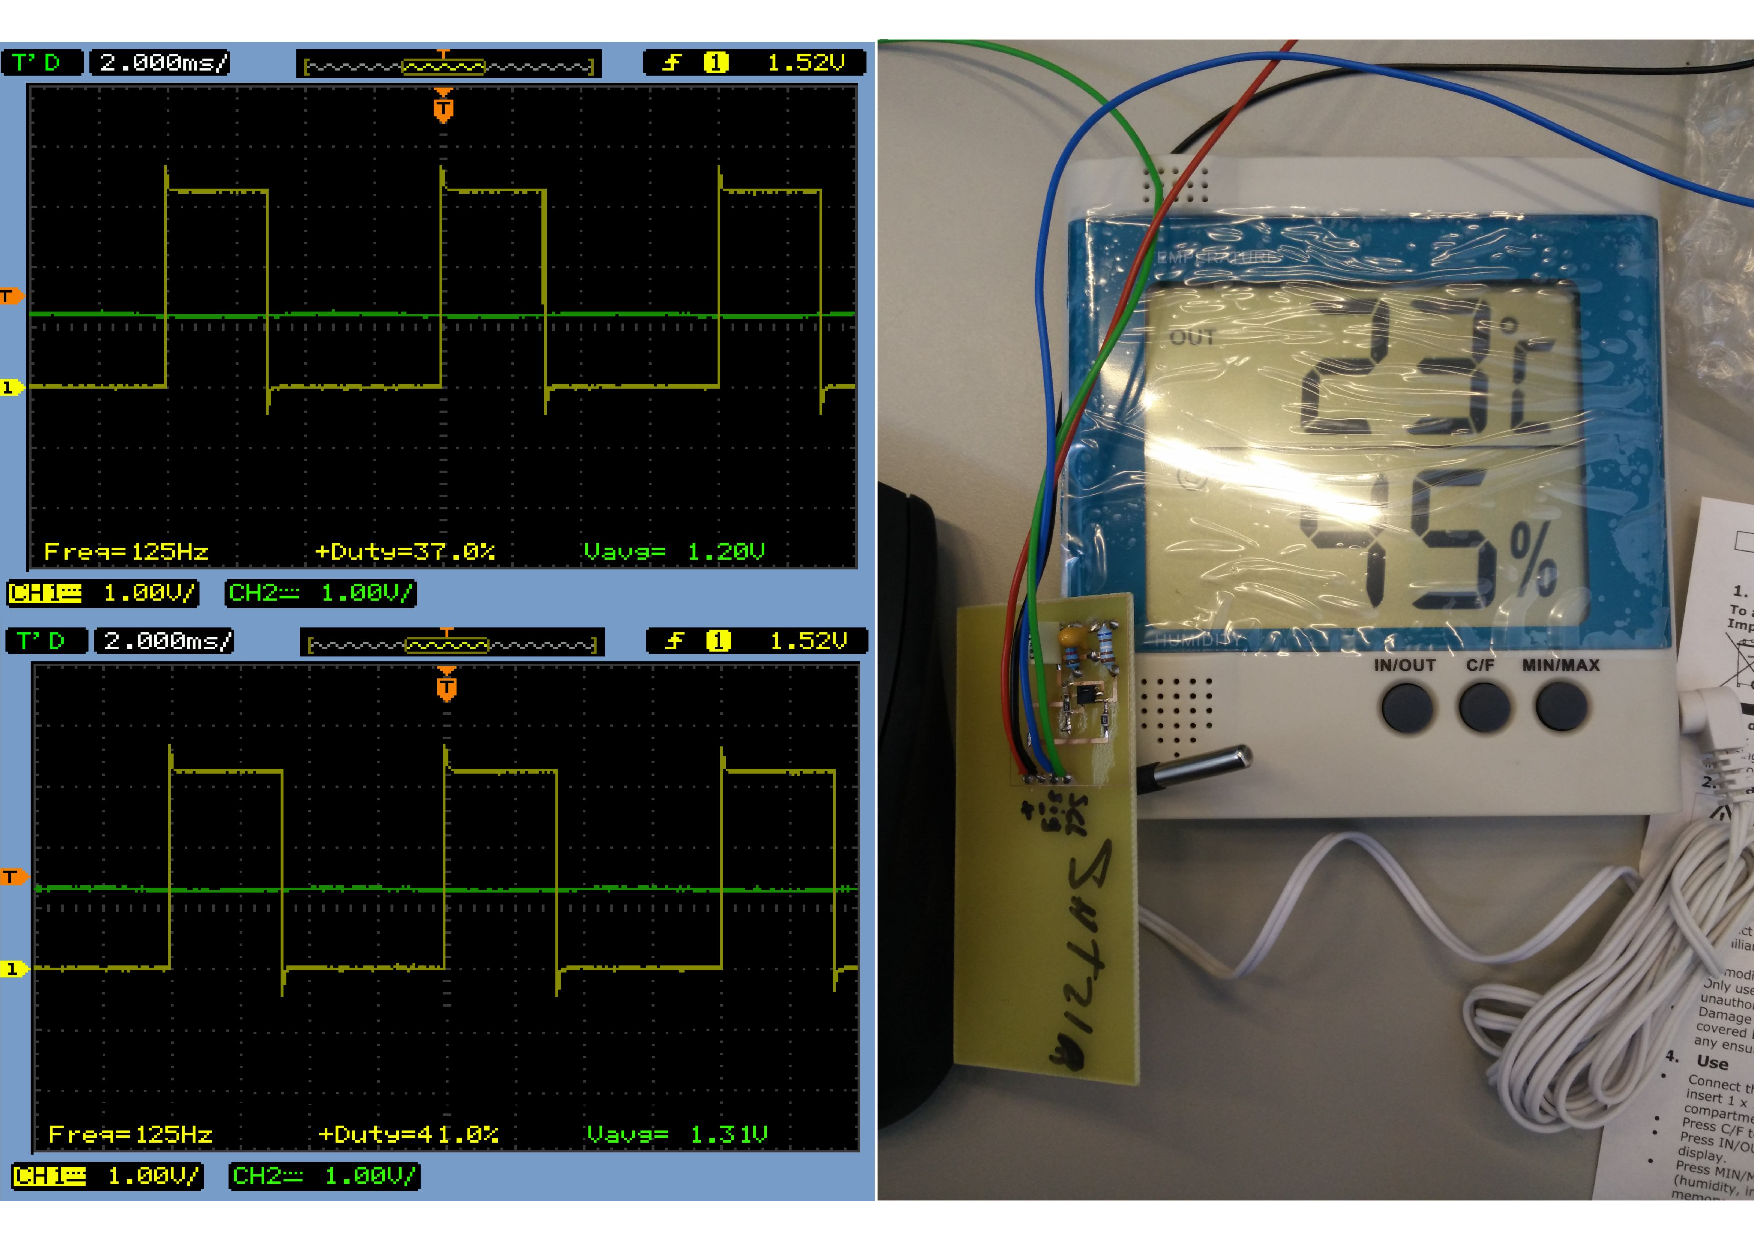
\includegraphics[width=0.90\textwidth]{filer/modultest/Billeder/test_stue}}
\caption{Billede af test ved stuetemperatur incl. oscilloskop billede, øverste scopbillede er fugtighed og nederste er temperatur}
\label{lab:test_stue}
\end{figure}

Som figur \ref{lab:test_stue} viser måles både en DC- og et PWM-signal. DCen er signalet efter lavpasfilteret og PWMen er den rå data fra sensoren. 
Sensorens SCL-ben er sat højt og sensoren måler derfor fugtighed. PWMen måles til at have en duty cycle på 37 \% og spændingen efter filteret måles til 1,2 V. Ud fra databladet kan duty cyclen omregnes til fugtighed med følgende formel:

Fugtighed regnet ud fra duty cycle
\begin{equation}
-6+125*0.37=40,25\%
\end{equation}

Med følende formel regnes fugtigheden ud fra DC-værdien.
\begin{equation}
-6+125*\frac{1,2}{3,28}= 39,73\%
\end{equation}

SCL-benet ligges nu lav og temperaturen måles ved at for.Ud fra PWM regnes nu temperaturen. PWMen måles til at have en duty cycle på 41 \% og en spænding efter filteret på 1.31 V. 

\begin{equation}
-46.85+175.72*0,41=25.2
\end{equation}

Temperaturen regnes ud fra DCen som følger. 

\begin{equation}
-46.85+175.72*\frac{1,31}{3,28}=23.33
\end{equation}


For at teste andre forhold bruges en varmepistol til at hæve temperatur og sænke fugtigheden. 
Samme målinger foretages:

\begin{figure}[h]
\centering
{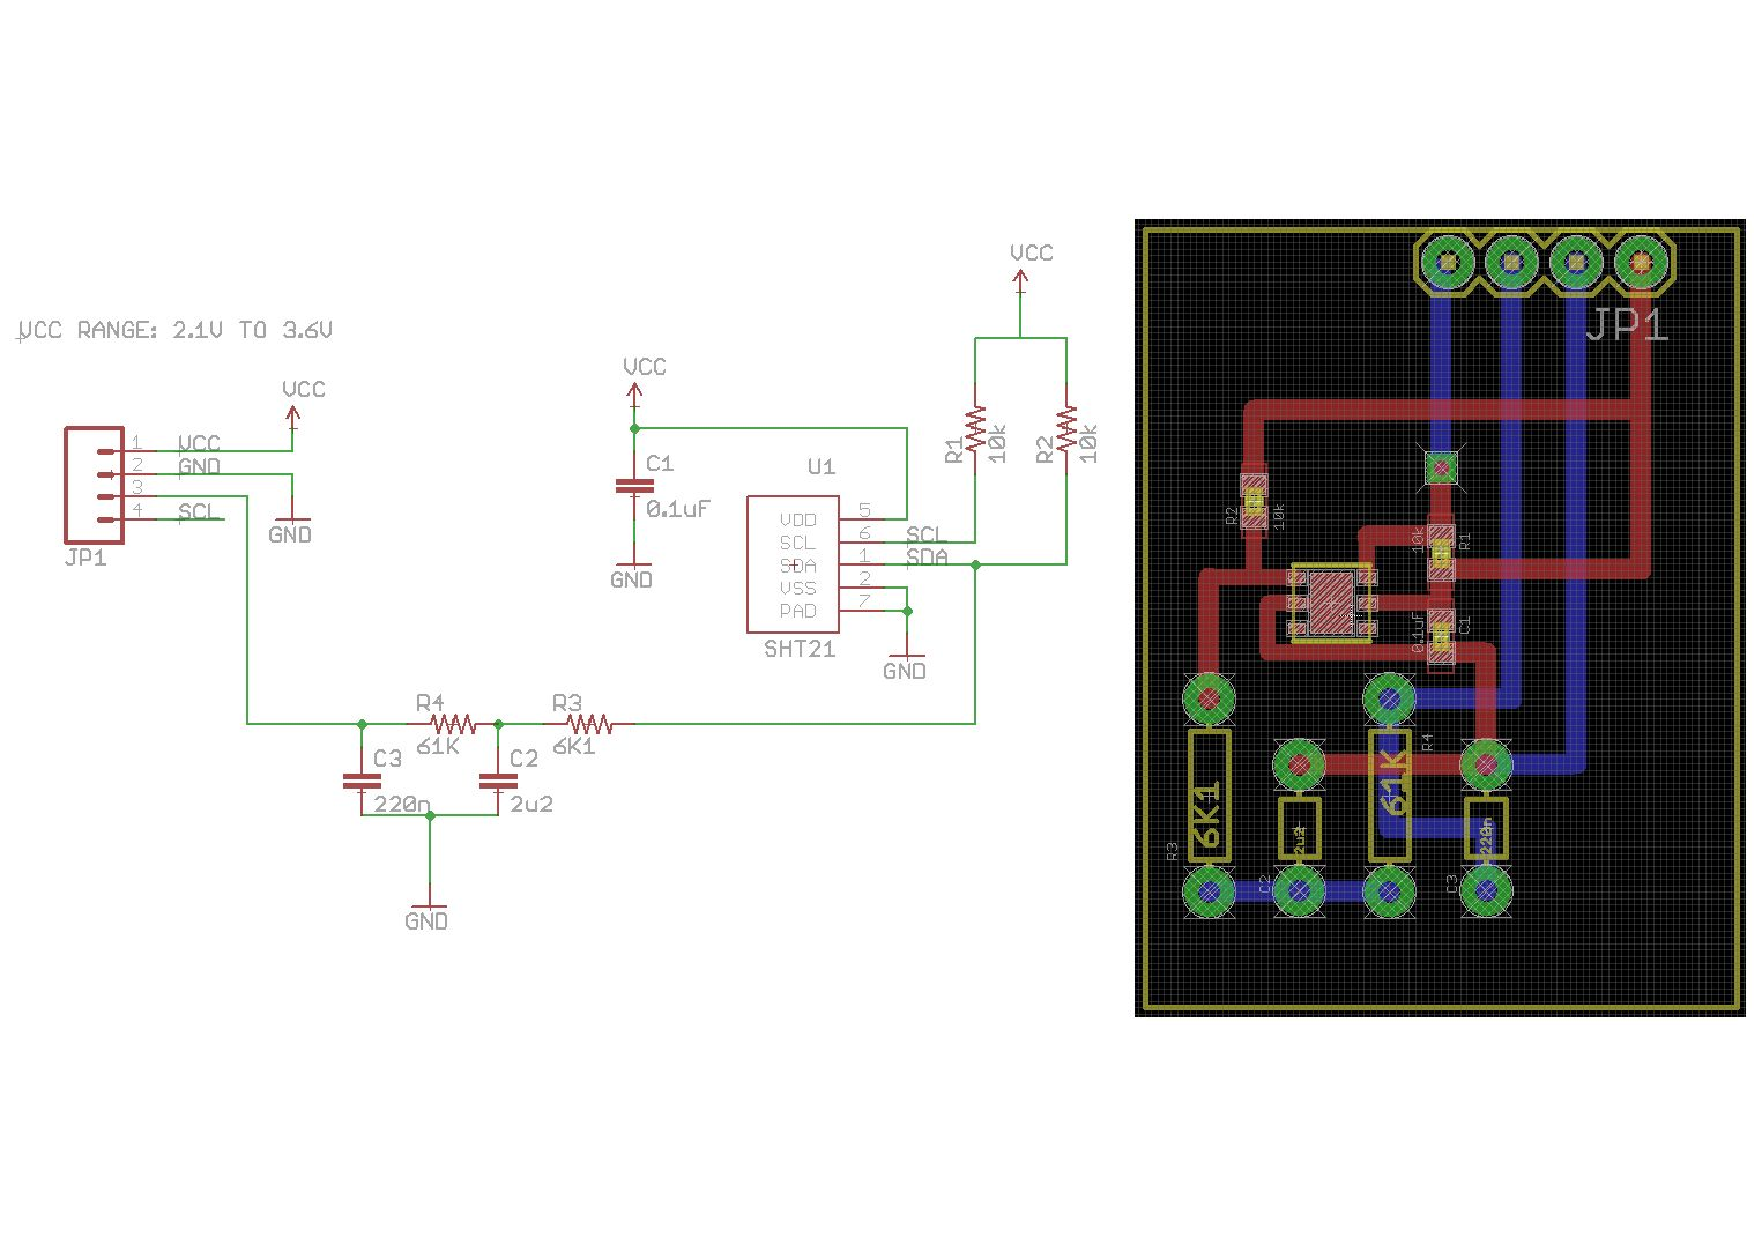
\includegraphics[width=0.90\textwidth]{filer/modultest/Billeder/test_varmt}}
\caption{Billede af test ved høj temperatur ink. oscilloskopbillede}
\label{lab:test_varmt}
\end{figure}

Igen regnes værdierne for temperatur og fugtighed ud fra PWMen med en dutycycle på 12,6 \% og DCen med en amplitude på 402 mV

\begin{equation}
-6+125*0,126= 9,75\%
\end{equation}

Med følgende formel regnes fugtigheden ud fra DC-værdien.

\begin{equation}
-6+125*\frac{0,402}{3,28}= 9,32\%
\end{equation}

SCL-benet sættes nu lavt ved at forbinde det til ground og temperaturen måles. Sensoren giver en PWM på 67,1 \% og en spænding efter filteret på 2,14 V. Ud fra PWM beregnes temperaturen.


\begin{equation}
-46.85+175.72*0,671=71,06
\end{equation}

Temperaturen regnes ud fra DCen som følger. 

\begin{equation}
-46.85+175.72*\frac{1,31}{3,28}=67,8
\end{equation}

For også at teste om sensoren kunne måle en høj luftfugtig foretages en måling efter at have åndet på sensoren. Da der allerede er målt temperatur ved både stuetemperatur og høj temperatur udelades temperaturtest af denne test. 

\begin{figure}[h]
\centering
{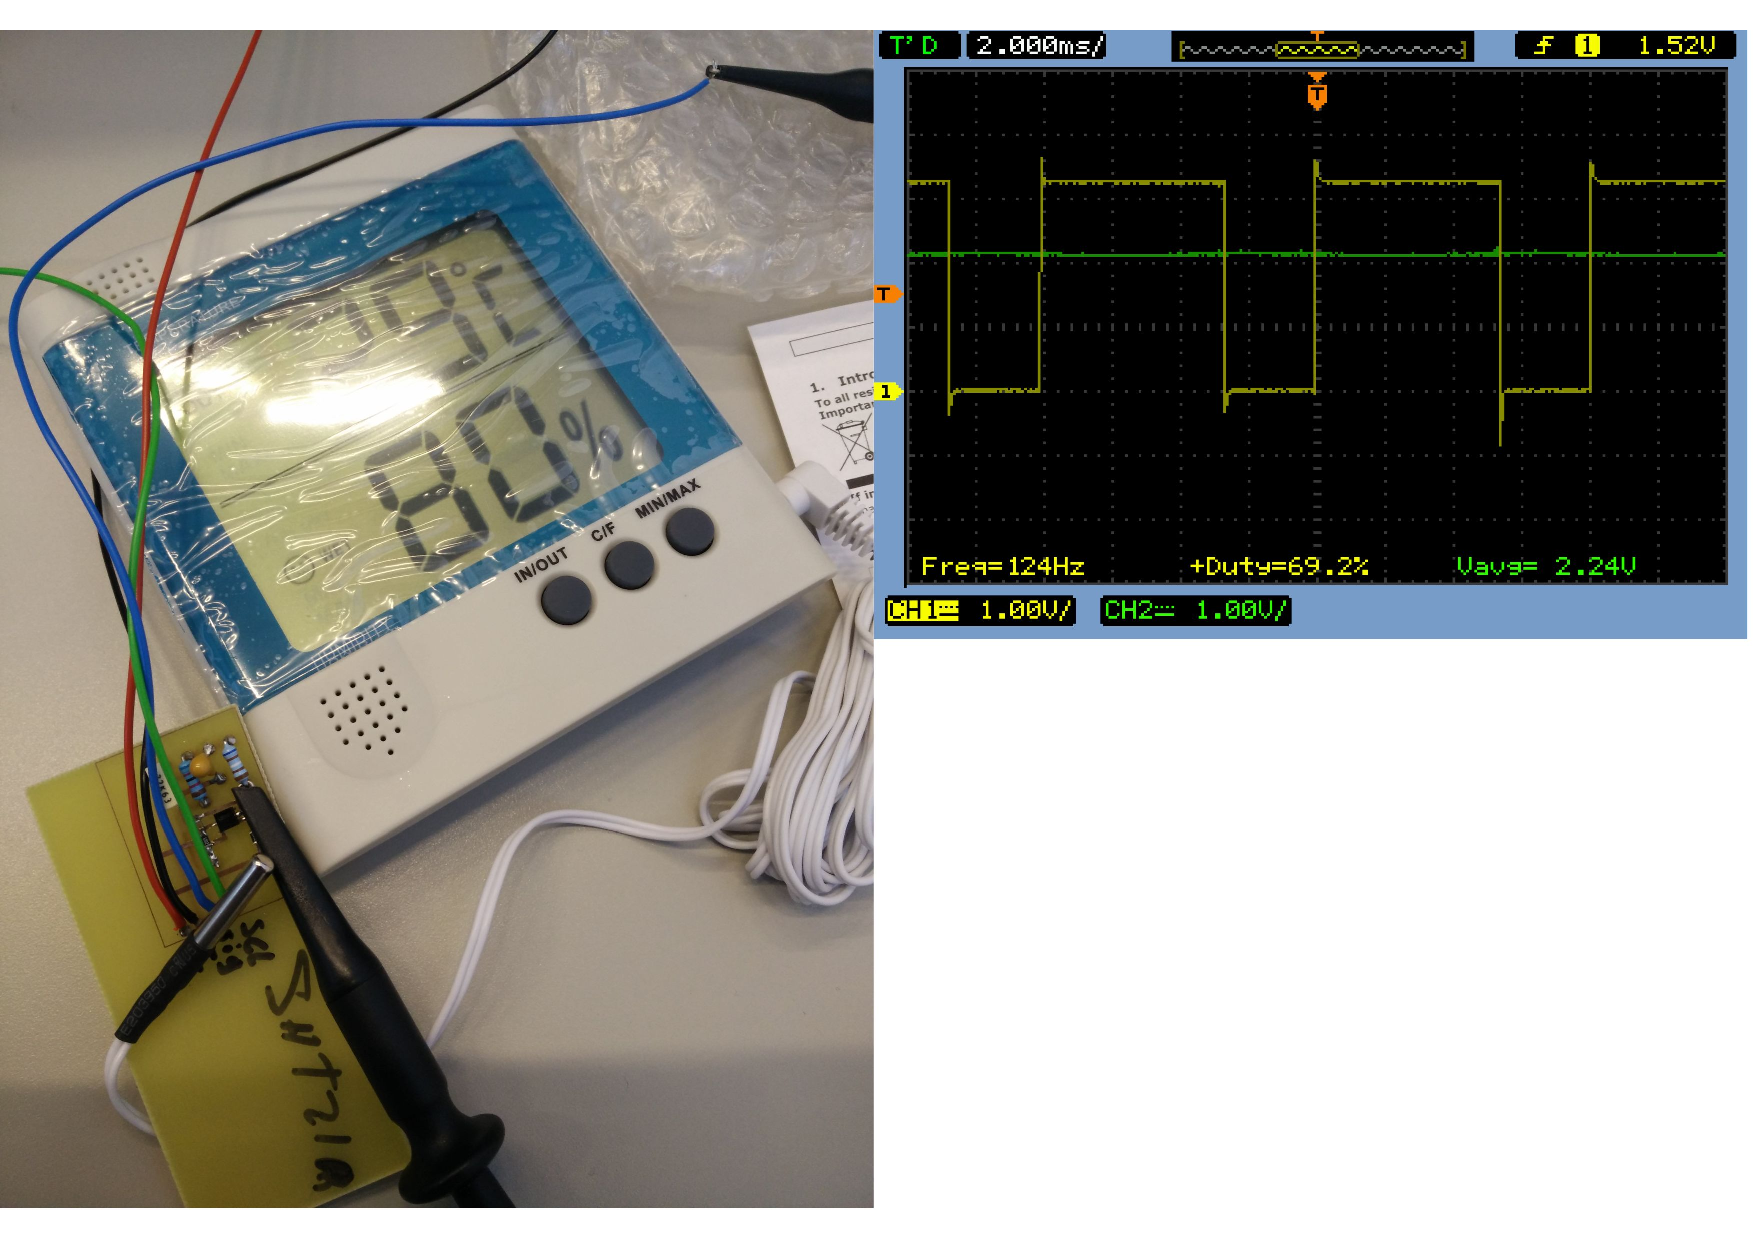
\includegraphics[width=0.90\textwidth]{filer/modultest/Billeder/test_fugtig}}
\caption{Billede af test med høj fugtighed incl oscilloskop billede}
\label{lab:test_fugtig}
\end{figure}

Ved testen sendte sensoren en PWM ud med en duty cycle på 69,2 \% og en spænding på 2,24 V efter filteret.


\begin{equation}
-6+125*0,692= 80,5\%
\end{equation}

Med følgende formel regnes fugtigheden ud fra DC-værdien.

\begin{equation}
-6+125*\frac{2,24}{3,28}= 79,37\%
\end{equation}


En test ved lav temperatur blev også fortaget. Temperaturen blev sænket ved hjælp af frysespray. Grundet den lave temperatur kom der kondensvand på sensoren som derfor målte en meget høj luftfugtighed. På grund af dette er måling af luftfugtighed udeladt af denne test. 


\begin{figure}[h]
\centering
{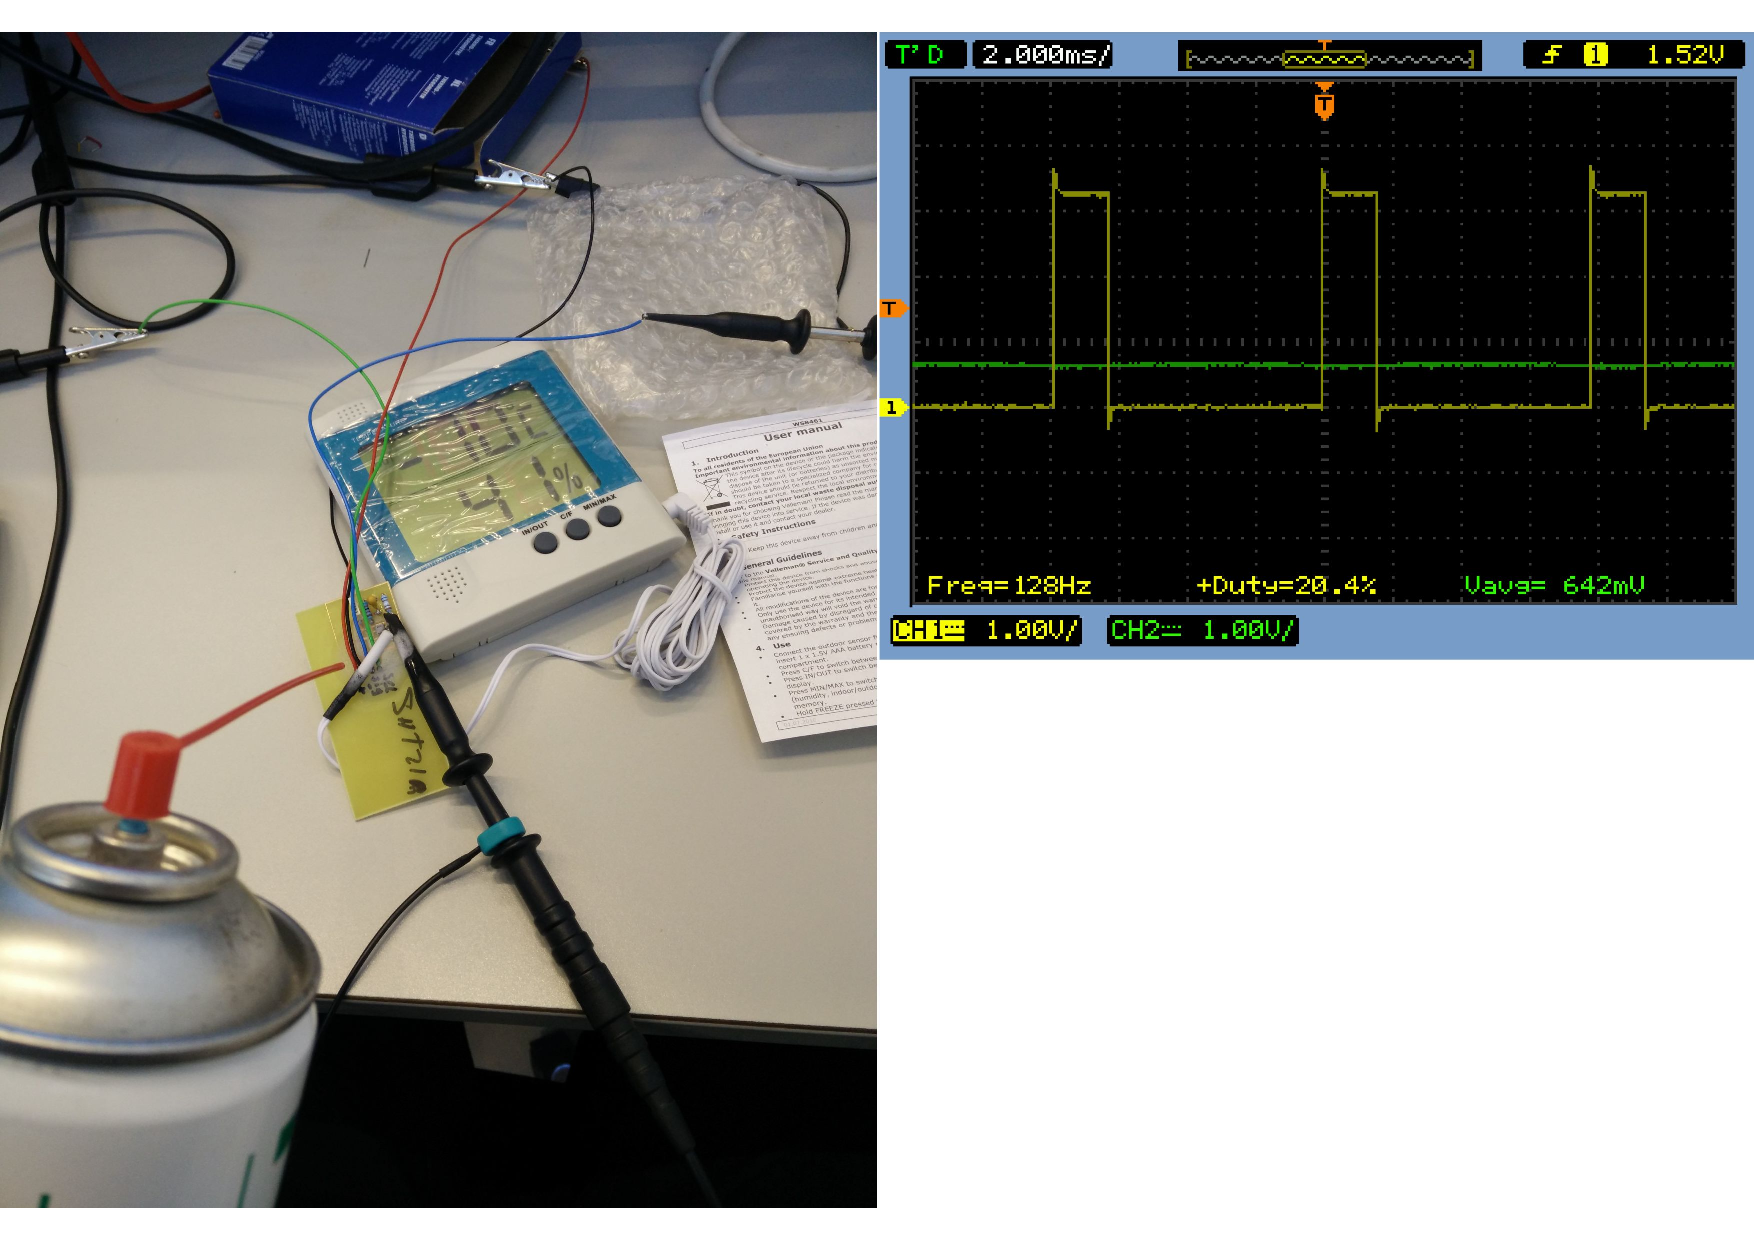
\includegraphics[width=0.90\textwidth]{filer/modultest/Billeder/test_kold}}
\caption{Billede af test med lav temperatur incl oscilloskop billede}
\label{lab:test_kold}
\end{figure}

Sensoren giver en PWM på 20,4 \% og en spænding efter filteret på 642 mV, temperatur beregnes herefter.


\begin{equation}
-46.85+175.72*0,204=11
\end{equation}

Temperaturen regnes ud fra DCen. 

\begin{equation}
-46.85+175.72*\frac{0,642}{3,28}=-12,66
\end{equation}

Grundet at det ikke var muligt at tage billede af den færdig temperatur og fugtighedsmåler og oscilloskopet samtidig godtages det at der er forskel på de to målinger og det skal derfor kun betrages som vejledende da der også var lang reaktionstid på den færdig måler mens SHT21P-sensoren ændrede sig øjeblikkeligt.
